\section{A Quick Example}\label{sec:example}

One of the most famous evolutionary games is that of Hawk-Dove\cite{maynard} which has been extended to multiple states by Eitan Altman et al\cite{markov5, markov3}. A simplified version of Altman's game (as presented in \cite{markov5}) is as follows:

\begin{itemize}[leftmargin=*,labelsep=4mm]
\item   $K = \{b\}$ A singular species of $b$ird
\item	$S=S_b = \{\mathbf{y},\mathbf{a},\mathbf{p}\}$ are the states of: $\mathbf{y}$oung, $\mathbf{a}$gressive adult, $\mathbf{p}$assive adult
\item	$A=A_b = \{R_\mathbf{a},R_\mathbf{p},G_\mathbf{a},G_\mathbf{p}\}$, $A_{b,\mathbf{y}}=\{G_\mathbf{a},G_\mathbf{p}\}$, $A_{b,\mathbf{p}}=\{R_\mathbf{p}\}$, $A_{b,\mathbf{a}}=\{R_\mathbf{a}\}$ are actions available to various states: $G_\mathbf{a}$/$G_\mathbf{p}$ is grow into aggressive/passive adult, $R_\mathbf{a}$/$R_\mathbf{p}$ is reproduce aggressively/passively.
\item   All the transmission rates are:\\
\begin{tabular}{cccc}
$T_{b,\mathbf{y},G_\mathbf{a}}(P^*_t)=0$ &
$T_{b,\mathbf{y},G_\mathbf{p}}(P^*_t)=0$ &
$T_{b,\mathbf{y},R_\mathbf{a}}(P^*_t)=2(1-p)$ &
$T_{b,\mathbf{y},R_\mathbf{p}}(P^*_t)=1-p+A$ \\
$T_{b,\mathbf{a},G_\mathbf{a}}(P^*_t)=1-pC$ &
$T_{b,\mathbf{a},G_\mathbf{p}}(P^*_t)=0$ &
$T_{b,\mathbf{a},R_\mathbf{a}}(P^*_t)=0$ &
$T_{b,\mathbf{a},R_\mathbf{p}}(P^*_t)=0$ \\
$T_{b,\mathbf{p},G_\mathbf{a}}(P^*_t)=DpC$ &
$T_{b,\mathbf{p},G_\mathbf{p}}(P^*_t)=DpC+1-pC$ &
$T_{b,\mathbf{p},R_\mathbf{a}}(P^*_t)=0$ &
$T_{b,\mathbf{p},R_\mathbf{p}}(P^*_t)=0$ \\
\end{tabular}
where $A,D,C$ are parameters of the game all between $0$ and $1$, and $p=\frac{P^*_{t,b,\mathbf{a},R_\mathbf{a}}}{P^*_{t,b,\mathbf{a},R_\mathbf{a}}+P^*_{t,b,\mathbf{p},R_\mathbf{p}}}$
\end{itemize}
It is noted that the only state which has multiple actions available to it is $\mathbf{y}$ with $G_\mathbf{a}$ and $G_\mathbf{p}$, and therefore the any strategy $w^b$ is totally specified once $\gamma = w^b_{G_\mathbf{a},\mathbf{y}}$ is specified, thus all strategies of the game can be parameterised by a single number $\gamma$, with $0\le\gamma\le 1$.\\
If the states are indexed in order $\mathbf{y},\mathbf{a},\mathbf{p}$ and the actions are indexed in order $R_\mathbf{a},R_\mathbf{p},G_\mathbf{a},G_\mathbf{p}$ then a strategy $w^b$ where $\gamma = w^b_{G_\mathbf{a},\mathbf{y}}$ has transmission matrix $m_{i,j}$ of the form:
\begin{equation}\label{eq:hd_transmission} m_{i,j} = \begin{bmatrix}
    0 & 2(1-p) & 1-p+A & \\
    \gamma(1-pC) & 0 & 0  & \\
     DpC+(1-\gamma)(1-pC)  & 0 & 0  & \\
\end{bmatrix} \end{equation}
The demographic flow of organisms of strategy $w^b$ between states can be visualised as per Figure \ref{fig:flow}.
\begin{figure}[]
\begin{center}
\begin{tikzpicture}[->,>=stealth']

    \node[state,anchor=center,text width=2cm]
        (Y) {Young};
    \node[state,anchor=center,text width=2cm,yshift=0.5cm,right of=Y,node distance=5.0cm]
        (A) {Aggressive\\Adult};
    \node[state,anchor=center,text width=2cm,yshift=-0.5cm,right of=Y,node distance=5.0cm]
        (P) {Passive\\Adult};

    \path (Y) edge[bend left=50]  node[anchor=south,above]{$\gamma(1-pC)$} (A);
    \path (A) edge[bend left=3]   node[anchor=south,above]{$2(1-p)$} (Y);
    \path (P) edge[bend left=-3]   node[anchor=south,below]{$1-p+A$} (Y);
    \path (Y) edge[bend left=-50] node[anchor=south,below]{$DpC+(1-\gamma)(1-pC)$} (P);

\end{tikzpicture}
\end{center}
\caption{A diagram of the flow of individual organisms between states of a simple Hawk-Dove game\\$\gamma$ being strategy parameter between $G_\mathbf{a}$ and $G_\mathbf{b}$, $p$ being proportion of Adults that are Aggressive, and $A$,$D$,$C$ being game parameters}
\label{fig:flow}
\end{figure}

We compared the results of the python software (of section \ref{sec:implementation}) on the Hawk-Dove game with those obtained by mathematical analysis (as given in Appendix \ref{appendix3}) and also via stochastic simulation.

The Moran process is a very simple stochastic model of the evolution of finite populations, wherein each 'turn' a random individual is chosen for reproduction proportional to its fitness and a corresponding random individual is chosen for death, the Moran process is generally regarded as a cornerstone technique of stochastic evolutionary game dynamics.\cite{stochastic1}

A Moran process for the above game is programmed (with source-code shown in Appendix \ref{appendix4}) and the results of the Moran process against the python implementation and mathematical analysis are shown in figure \ref{fig:bigfigure}.
The figure shows the value $p$ (the proportion of adults that are aggressive) and the proportion of young ($\%Y$) at equilibrium against the parameter $A$ for fixed $C$ and $D$ and shows a strong coincidence in achieving a non-trivial result for all three methodologies.

\begin{figure}[]
\begin{center}
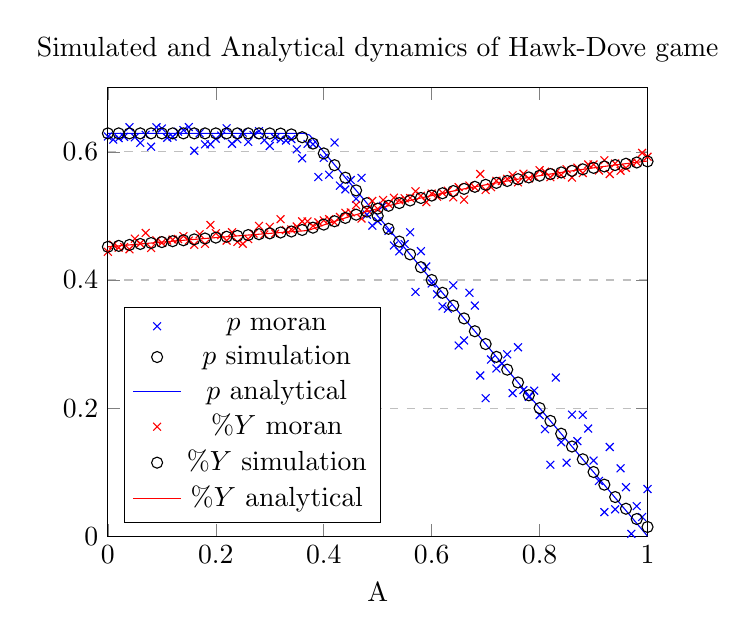
\begin{tikzpicture}
\begin{axis}[
    title={Simulated and Analytical dynamics of Hawk-Dove game},
    xlabel={A},
    xmin=0, xmax=1,
    ymin=0, ymax=0.7,
    xtick={0,0.2,0.4,0.6,0.8,1.0},
    ytick={0,0.2,0.4,0.6,0.8,1.0},
    legend pos=south west,
    ymajorgrids=true,
    grid style=dashed,
]
 
\addplot[
    color=blue,
    mark=x,
only marks,
    ]
    coordinates {
    (0.0,0.6241007194244604)(0.01,0.6192660550458715)(0.02,0.62147406733394)(0.03,0.6235186873290793)(0.04,0.6385869565217391)(0.05,0.6227824463118581)(0.06,0.6141804788213628)(0.07,0.6267806267806267)(0.08,0.6081818181818182)(0.09,0.6384758364312267)(0.1,0.6365313653136532)(0.11,0.6220984215413184)(0.12,0.6238361266294227)(0.13,0.6315298507462687)(0.14,0.6340545625587959)(0.15,0.6388115134633241)(0.16,0.6018348623853211)(0.17,0.6291390728476821)(0.18,0.6117755289788408)(0.19,0.6118677042801557)(0.2,0.6204933586337761)(0.21,0.6254716981132076)(0.22,0.6369545032497679)(0.23,0.6127497621313035)(0.24,0.6197964847363552)(0.25,0.6301747930082797)(0.26,0.6156716417910447)(0.27,0.6265402843601896)(0.28,0.6323957322987391)(0.29,0.6181474480151229)(0.3,0.6092843326885881)(0.31,0.6218009478672986)(0.32,0.6198019801980198)(0.33,0.617816091954023)(0.34,0.6199616122840691)(0.35000000000000003,0.6040658276863504)(0.36,0.5899705014749262)(0.37,0.6125860373647984)(0.38,0.612027158098933)(0.39,0.5607843137254902)(0.4,0.5907297830374754)(0.41000000000000003,0.5643564356435643)(0.42,0.6147058823529412)(0.43,0.5473579262213359)(0.44,0.5414141414141415)(0.45,0.5561172901921132)(0.46,0.5269151138716356)(0.47000000000000003,0.5595238095238095)(0.48,0.5020408163265306)(0.49,0.48478488982161594)(0.5,0.4918200408997955)(0.51,0.5157894736842106)(0.52,0.4766355140186916)(0.53,0.45387062566277836)(0.54,0.444794952681388)(0.55,0.4560846560846561)(0.56,0.4745762711864407)(0.5700000000000001,0.38136511375947996)(0.58,0.4450373532550694)(0.59,0.4211076280041797)(0.6,0.3946236559139785)(0.61,0.3776595744680851)(0.62,0.3588362068965517)(0.63,0.3550488599348534)(0.64,0.39171974522292996)(0.65,0.2978021978021978)(0.66,0.3055848261327713)(0.67,0.38011049723756907)(0.68,0.3600439077936334)(0.6900000000000001,0.2508630609896433)(0.7000000000000001,0.21545157780195864)(0.71,0.27582417582417584)(0.72,0.26179775280898876)(0.73,0.26936026936026936)(0.74,0.2839366515837104)(0.75,0.22336769759450173)(0.76,0.29497206703910617)(0.77,0.22811059907834103)(0.78,0.217440543601359)(0.79,0.2271689497716895)(0.8,0.18903150525087514)(0.81,0.16705336426914152)(0.8200000000000001,0.11149032992036405)(0.8300000000000001,0.24768518518518517)(0.84,0.14678899082568808)(0.85,0.11475409836065574)(0.86,0.18977272727272726)(0.87,0.14840989399293286)(0.88,0.18937644341801385)(0.89,0.16805721096543505)(0.9,0.11799761620977355)(0.91,0.08624708624708624)(0.92,0.03753026634382567)(0.93,0.13924050632911392)(0.9400000000000001,0.041866028708133975)(0.9500000000000001,0.10593713620488941)(0.96,0.07647058823529412)(0.97,0.0035971223021582736)(0.98,0.046875)(0.99,0.029887920298879204)(1.0,0.0736196319018405)
    };
\addlegendentry{$p$ moran}
\addplot[
    color=black,
    mark=o,
only marks,
    ]
    coordinates {
(0,0.6289575466)(0.02,0.6289575466)(0.04,0.6289575466)(0.06,0.6289575466)(0.08,0.6289575466)(0.1,0.6289575466)(0.12,0.6289575466)(0.14,0.6289575466)(0.16,0.6289575466)(0.18,0.6289575465)(0.2,0.6289575451)(0.22,0.6289575318)(0.24,0.6289574112)(0.26,0.6289564175)(0.28,0.6289490304)(0.3,0.6289001852)(0.32,0.6286217323)(0.34,0.6273346255)(0.36,0.622964624)(0.38,0.6130200741)(0.4,0.5976515858)(0.42,0.5792825877)(0.44,0.5597835311)(0.46,0.539932344)(0.48,0.5199776121)(0.5,0.4999921004)(0.52,0.4799970362)(0.54,0.4599988331)(0.56,0.4399995329)(0.58,0.4199998251)(0.6,0.3999999577)(0.62,0.3800000258)(0.64,0.360000069)(0.66,0.3400001064)(0.68,0.3200001504)(0.7,0.3000002138)(0.72,0.2800003163)(0.74,0.2600004944)(0.76,0.2400008227)(0.78,0.2200014619)(0.8,0.2000027757)(0.82,0.1800056245)(0.84,0.1600121288)(0.86,0.1400277109)(0.88,0.1200666434)(0.9,0.1001671363)(0.92,0.0804311295)(0.94,0.0611204033)(0.96,0.0428443188)(0.98,0.0267625127)(1,0.0143807301)
    };
\addlegendentry{$p$ simulation}
\addplot [
    domain=0:1, 
    samples=100, 
    color=blue,
    ]
    {min(1-x,(-1*(0.7+1)+sqrt((0.7+1)^2+4*(0.75*0.7-0.7)))/(2*(0.75*0.7-0.7)))};
\addlegendentry{$p$ analytical}

\addplot[
    color=red,
    mark=x,
only marks,
    ]
    coordinates {
    (0.0,0.444)(0.01,0.455)(0.02,0.4505)(0.03,0.4515)(0.04,0.448)(0.05,0.4645)(0.06,0.457)(0.07,0.4735)(0.08,0.45)(0.09,0.462)(0.1,0.458)(0.11,0.4615)(0.12,0.463)(0.13,0.464)(0.14,0.4685)(0.15,0.4615)(0.16,0.455)(0.17,0.4715)(0.18,0.4565)(0.19,0.486)(0.2,0.473)(0.21,0.47)(0.22,0.4615)(0.23,0.4745)(0.24,0.4595)(0.25,0.4565)(0.26,0.464)(0.27,0.4725)(0.28,0.4845)(0.29,0.471)(0.3,0.483)(0.31,0.4725)(0.32,0.495)(0.33,0.478)(0.34,0.479)(0.35000000000000003,0.4835)(0.36,0.4915)(0.37,0.4915)(0.38,0.4845)(0.39,0.49)(0.4,0.493)(0.41000000000000003,0.495)(0.42,0.49)(0.43,0.4985)(0.44,0.505)(0.45,0.5055)(0.46,0.517)(0.47000000000000003,0.496)(0.48,0.51)(0.49,0.5235)(0.5,0.511)(0.51,0.525)(0.52,0.5185)(0.53,0.5285)(0.54,0.5245)(0.55,0.5275)(0.56,0.528)(0.5700000000000001,0.5385)(0.58,0.5315)(0.59,0.5215)(0.6,0.535)(0.61,0.53)(0.62,0.536)(0.63,0.5395)(0.64,0.529)(0.65,0.545)(0.66,0.5255)(0.67,0.5475)(0.68,0.5445)(0.6900000000000001,0.5655)(0.7000000000000001,0.5405)(0.71,0.545)(0.72,0.555)(0.73,0.5545)(0.74,0.558)(0.75,0.5635)(0.76,0.5525)(0.77,0.566)(0.78,0.5585)(0.79,0.562)(0.8,0.5715)(0.81,0.569)(0.8200000000000001,0.5605)(0.8300000000000001,0.568)(0.84,0.564)(0.85,0.573)(0.86,0.56)(0.87,0.5755)(0.88,0.567)(0.89,0.5805)(0.9,0.5805)(0.91,0.571)(0.92,0.587)(0.93,0.5655)(0.9400000000000001,0.582)(0.9500000000000001,0.5705)(0.96,0.575)(0.97,0.583)(0.98,0.584)(0.99,0.5985)(1.0,0.5925)
    };
\addlegendentry{$\%Y$ moran}

\addplot[
    color=black,
    mark=o,
only marks,
    ]
    coordinates {
(0,0.4517891488)(0.02,0.4533007859)(0.04,0.4547950448)(0.06,0.4562723037)(0.08,0.4577329282)(0.1,0.4591772724)(0.12,0.4606056792)(0.14,0.4620184805)(0.16,0.4634159981)(0.18,0.4647985439)(0.2,0.4661664205)(0.22,0.467519924)(0.24,0.4688593629)(0.26,0.4701852059)(0.28,0.4714991067)(0.3,0.4728101081)(0.32,0.4741654624)(0.34,0.4757588605)(0.36,0.4780953866)(0.38,0.4817321369)(0.4,0.4865074548)(0.42,0.4917375503)(0.44,0.4969566765)(0.46,0.501998492)(0.48,0.5068270573)(0.5,0.5114452157)(0.52,0.5158650917)(0.54,0.5201001195)(0.56,0.52416307)(0.58,0.5280656464)(0.6,0.5318184805)(0.62,0.5354312238)(0.64,0.5389126531)(0.66,0.5422707686)(0.68,0.5455128809)(0.7,0.5486456873)(0.72,0.5516753368)(0.74,0.5546074882)(0.76,0.5574473581)(0.78,0.5601997623)(0.8,0.5628691478)(0.82,0.565459611)(0.84,0.567974887)(0.86,0.5704182752)(0.88,0.5727924)(0.9,0.5750985588)(0.92,0.5773350747)(0.94,0.5794935866)(0.96,0.5815525074)(0.98,0.583471595)(1,0.5852028369)
    };
\addlegendentry{$\%Y$ simulation}

\addplot [
    domain=0:1, 
    samples=100, 
    color=red,
    ]
    {max(sqrt(2*x)/(sqrt(2*x)+sqrt(0.7*(1-x)*(0.75-1)+1)), (sqrt(0.75*0.6289575465860742*0.7*(1+0.6289575465860742+x)))/(sqrt(0.75*0.6289575465860742*0.7*(1+0.6289575465860742+x))+1-0.6289575465860742*0.7+0.75*0.6289575465860742*0.7))};
\addlegendentry{$\%Y$ analytical}
 
\end{axis}
\end{tikzpicture}
\caption{Dynamics of the Hawk-Dove game across parameter $A$, with $D = 0.75$ and $C = 0.70$\\ shown are results for $p$ as well as proportion Young $\%Y$ for Moran stochastic simulation, analytical prediction, and our software solver's results}
\label{fig:bigfigure}
\end{center}
\end{figure}

